% Sections: the three acts of the results. NOT drafted yet (docs/paper_outline.md sections 4-6). The tables and the
% figure below are generated from committed results (scripts/paper/build.py) and placed where the text will use them.
\section{Optimization: $\sigma$ rides on the answer's advantage}
\label{sec:act1}
\todo{To be written (docs/paper\_outline.md, section 4; FINDINGS \#6, \#14, \#16, \#18, \#25).}

\begin{figure}[t]
  \centering
  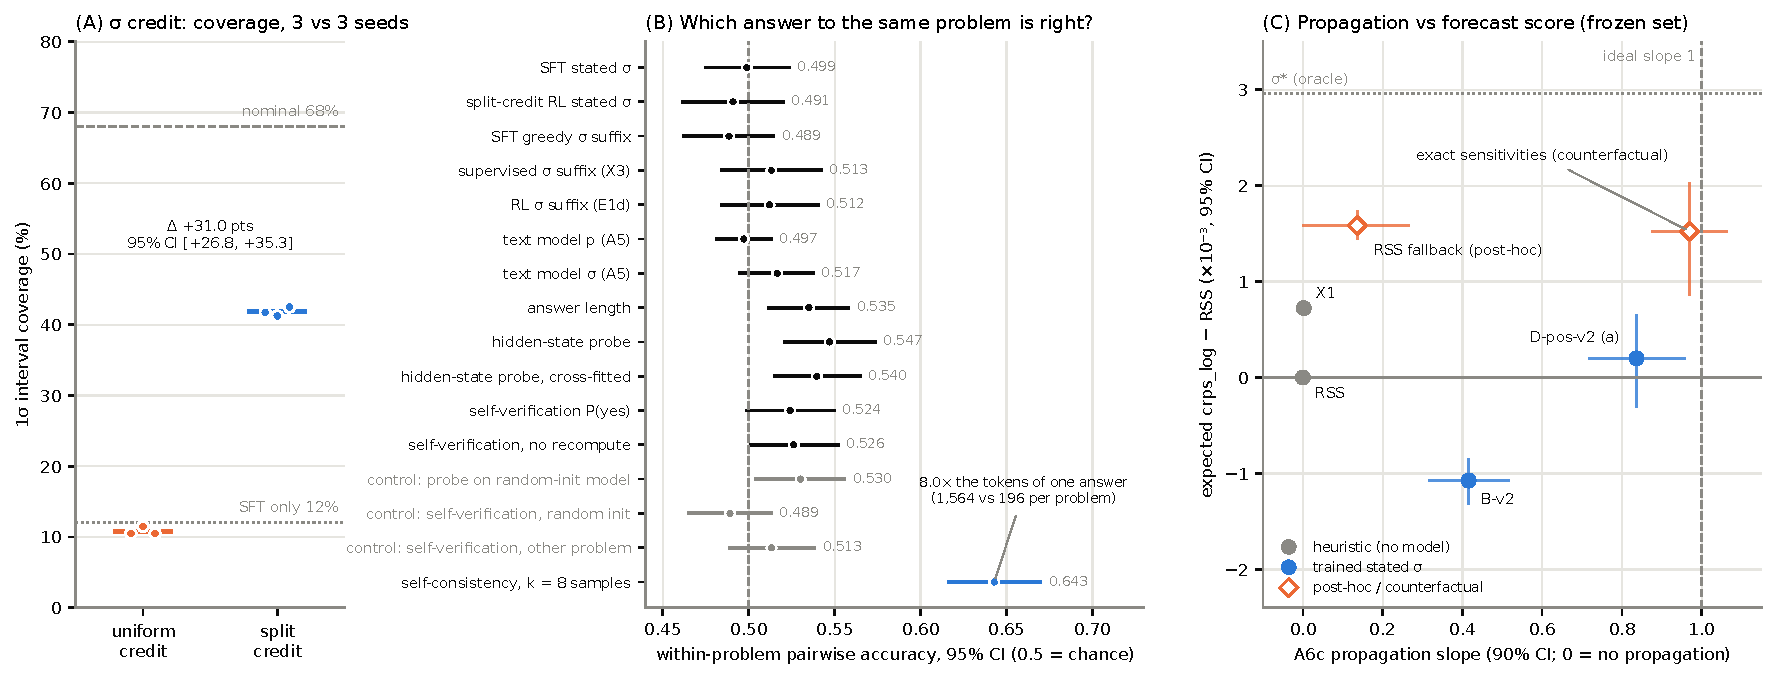
\includegraphics[width=\linewidth]{generated/figures/headline.pdf}
  % scripts/figures/headline.py via scripts/paper/figures.py; sources in paper/generated/SOURCES.md
  % (fig_headline); FINDINGS #18 (A), #19, #21, #22, #26, #37 (B), #32, #35, #36 (C).
  \caption{The three findings.
  (A) Uniform versus split credit: $1\sigma$ coverage per seed.
  (B) Within-problem pairwise accuracy of every correctness readout measured, against self-consistency.
  (C) On the frozen set, the noise-allocation slope against the expected-score difference from RSS.
  Every point is read from a committed result file; the sidecar \texttt{headline\_data.json} traces each one.}
  \label{fig:headline}
\end{figure}

\section{Does the model know which of its answers is right?}
\label{sec:act2}
\todo{To be written (docs/paper\_outline.md, section 5; FINDINGS \#7, \#19--\#22, \#26, \#37).}

% GENERATED by scripts/paper/tables.py; do not edit. Rebuild: uv run python scripts/paper/build.py
% artifact: table:cost
% sources (path @ git blob):
%   results/r5_diag/cost.json @ 364d31ae15dd
\begin{table}[t]
\centering
\small
\caption{Correctness signals against their inference cost.}
\label{tab:cost}
\begin{tabular}{@{}L{6.4cm} l r@{}}
\toprule
readout & pairwise accuracy [95\% CI] & tokens / problem \\
\midrule
self-consistency (agreement of the other samples) & \num{0.643} [\num{0.616}, \num{0.671}] & \num{1564} \\
hidden-state probe & \num{0.547} [\num{0.520}, \num{0.574}] & \num{196} \\
the same probe, random-init model & \num{0.530} [\num{0.503}, \num{0.557}] & \num{196} \\
completion length & \num{0.535} [\num{0.511}, \num{0.559}] & \num{196} \\
self-verification P(yes) (X4) & \num{0.524} [\num{0.498}, \num{0.550}] & \num{196} \\
stated $\sigma$ (SFT) & \num{0.499} [\num{0.474}, \num{0.524}] & \num{196} \\
\bottomrule
\end{tabular}
\par\smallskip\begin{minipage}{0.95\linewidth}\footnotesize Within-problem pairwise accuracy (a right answer ranked above a wrong one to the same problem; \num{516} problems, 95\% CIs clustered over problems) against generated tokens per problem (k = \num{8} samples for self-consistency). Source: results/r5\_diag/cost.json (FINDINGS \#22, \#37).\end{minipage}
\end{table}

% GENERATED by scripts/paper/tables.py; do not edit. Rebuild: uv run python scripts/paper/build.py
% artifact: table:cost_mca
% sources (path @ git blob):
%   results/r5_diag/cost.json @ 364d31ae15dd
\begin{table}[t]
\centering
\small
\caption{MC-A's spread against its cost, and MC-B's failure split.}
\label{tab:costmca}
\begin{tabular}{@{}l r r@{}}
\toprule
signal & AUROC & extra tokens / problem \\
\midrule
$\sigma^\star$ & \num{0.665} & \num{0} \\
RSS & \num{0.654} & \num{0} \\
X1 & \num{0.666} & \num{0} \\
B-v2 stated $\sigma$ & \num{0.655} & \num{0} \\
MC-A raw spread, $k=\num{2}$ & \num{0.638} & \num{496} \\
MC-A raw spread, $k=\num{4}$ & \num{0.710} & \num{992} \\
MC-A raw spread, $k=\num{8}$ & \num{0.745} & \num{1984} \\
\bottomrule
\end{tabular}
\par\smallskip\begin{minipage}{0.95\linewidth}\footnotesize A6c (development), AUROC of the signal for B-v2's run-0 answer being wrong, against the extra generated tokens per problem. MC-B's programs on the same set: \SI{79.7}{\percent} fail at the interface, \SI{5.1}{\percent} at run time, \SI{14.7}{\percent} run but compute the wrong chain, \SI{0.5}{\percent} are correct. Source: results/r5\_diag/cost.json (FINDINGS \#31, \#33, \#37).\end{minipage}
\end{table}


\section{Propagation of measurement noise: structure is not forecast quality}
\label{sec:act3}
\todo{To be written (docs/paper\_outline.md, section 6; FINDINGS \#17, \#23, \#27--\#39).}

% GENERATED by scripts/paper/tables.py; do not edit. Rebuild: uv run python scripts/paper/build.py
% artifact: table:confirmatory
% sources (path @ git blob):
%   results/stage_r4/confirmatory/results.json @ dc002a81d4ba
\begin{table}[t]
\centering
\small
\caption{The R4-3 confirmatory run: D-pos-v2 and B-v2 on the frozen set.}
\label{tab:confirmatory}
\begin{tabular}{@{}l L{5.2cm} l l l@{}}
\toprule
test & statistic & estimate [90\% CI] & $p$ & Holm \\
\midrule
K1 & D-pos-v2 (a): A6c slope $>0$ (primary) & \num{+0.816} [\num{+0.707}, \num{+0.923}] & \num{<1e-4} & rejected \\
K2 & D-pos-v2 (b) line's $X$: A6c slope $>0$ & \num{+0.884} [\num{+0.745}, \num{+1.041}] & \num{<1e-4} & rejected \\
K3 & D-pos-v2 (c) exact from terms: A6c slope $>0$ & \num{+0.843} [\num{+0.713}, \num{+0.987}] & \num{<1e-4} & rejected \\
K4 & B-v2: A6c slope $>0$ & \num{+0.416} [\num{+0.315}, \num{+0.517}] & \num{<1e-4} & rejected \\
K5 & D-pos-v2 $-$ B-v2 (expected crps\_log) & \num{+0.0013} [\num{+0.0008}, \num{+0.0017}] & \num{<1e-4} & rejected \\
K6 & D-pos-v2 $-$ RSS & \num{+0.0002} [\num{-0.0002}, \num{+0.0006}] & \num{0.201} & -- \\
K7 & D-pos-v2 $-$ X1 & \num{-0.0005} [\num{-0.0009}, \num{-0.0001}] & \num{0.991} & -- \\
K8 & B-v2 $-$ RSS & \num{-0.0011} [\num{-0.0013}, \num{-0.0009}] & \num{1.000} & -- \\
\midrule
C1--C3 & D-pos-v2 (a): A6b slope \num{+0.036} [\num{-0.057}, \num{+0.212}] & C1 yes, C2 yes, C3 yes & &  \\
C1--C3 & D-pos-v2 (b): A6b slope \num{-0.026} [\num{-0.049}, \num{-0.007}] & C1 yes, C2 yes, C3 yes & &  \\
C1--C3 & D-pos-v2 (c): A6b slope \num{-0.023} [\num{-0.047}, \num{-0.005}] & C1 yes, C2 yes, C3 yes & &  \\
C1--C3 & B-v2 (a): A6b slope \num{+0.003} [\num{-0.086}, \num{+0.129}] & C1 yes, C2 no, C3 yes & &  \\
\bottomrule
\end{tabular}
\par\smallskip\begin{minipage}{0.95\linewidth}\footnotesize Seed means over \num{3} seeds per arm, frozen R4-5 set (\num{3060} problems); stage B's joint pairs bootstrap, $B=\num{10000}$; 90\% CIs; one-sided $p$; Holm over K1--K8 at 0.05. Expected-score rows: oracle-centred expected crps\_log, pooled over the three sets, clustered over pairs. P = K1 $\wedge$ C2 $\wedge$ C3 (D125): confirmed. Source: results/stage\_r4/confirmatory/results.json (D118, D125; FINDINGS \#32).\end{minipage}
\end{table}

% GENERATED by scripts/paper/tables.py; do not edit. Rebuild: uv run python scripts/paper/build.py
% artifact: table:tail
% sources (path @ git blob):
%   results/r5_diag/tail.json @ d92087ff65fd
\begin{table}[t]
\centering
\small
\caption{Tail autopsy: what the worst problems get wrong.}
\label{tab:tail}
\begin{tabular}{@{}l r r@{}}
\toprule
primary cause & problem-seeds & share \\
\midrule
sensitivity: value-dependent: formula & \num{177} & \SI{39}{\percent} \\
sensitivity: value-dependent: substitution (own wrong intermediates) & \num{87} & \SI{19}{\percent} \\
copy: decimal shift & \num{71} & \SI{16}{\percent} \\
chain selection: wrong number of terms & \num{35} & \SI{8}{\percent} \\
sensitivity: power-law exponent & \num{28} & \SI{6}{\percent} \\
format: no answer $\sigma$ & \num{26} & \SI{6}{\percent} \\
sensitivity: value-dependent: formula (no expression) & \num{18} & \SI{4}{\percent} \\
format: no parsable $\sigma$ line & \num{7} & \SI{2}{\percent} \\
aggregation & \num{5} & \SI{1}{\percent} \\
sensitivity: transcription (S line right, $\sigma$-line coefficient wrong) & \num{1} & \SI{0}{\percent} \\
sensitivity: value-dependent: substitution (values) & \num{1} & \SI{0}{\percent} \\
\bottomrule
\end{tabular}
\par\smallskip\begin{minipage}{0.95\linewidth}\footnotesize D-pos-v2 (a), frozen R4-5 set, \num{3} seeds; the worst 5\% of problems by regret against $\sigma^\star$ per seed (\num{456} problem-seeds), classified by primary cause. They hold \SI{69}{\percent}--\SI{83}{\percent} of each seed's regret. Descriptive (R5-2, D133). Source: results/r5\_diag/tail.json (FINDINGS \#35).\end{minipage}
\end{table}

% GENERATED by scripts/paper/tables.py; do not edit. Rebuild: uv run python scripts/paper/build.py
% artifact: table:swaps
% sources (path @ git blob):
%   results/r5_diag/tail.json @ d92087ff65fd
\begin{table}[t]
\centering
\small
\caption{Component swaps: which part of the explicit $\sigma$ costs the score.}
\label{tab:swaps}
\begin{tabular}{@{}L{6.2cm} l r r@{}}
\toprule
$\sigma$ with & $-$ RSS [90\% CI] & gap closed & A6c slope \\
\midrule
(a) as stated & \num{+0.0002} [\num{-0.0002}, \num{+0.0006}] & \SI{7}{\percent} & \num{+0.837} \\
exact sensitivities (model's levels, aggregation, copy) & \num{+0.0015} [\num{+0.0010}, \num{+0.0020}] & \SI{51}{\percent} & \num{+0.970} \\
exact levels (model's sensitivities, aggregation, copy) & \num{+0.0002} [\num{-0.0002}, \num{+0.0006}] & \SI{7}{\percent} & \num{+0.838} \\
exact aggregation (model's terms and copy) & \num{-0.0008} [\num{-0.0016}, \num{-0.0001}] & \SI{-28}{\percent} & \num{+0.806} \\
exact copy, i.e. $\sigma$ = the line's X (= (b)) & \num{+0.0002} [\num{-0.0003}, \num{+0.0007}] & \SI{8}{\percent} & \num{+0.857} \\
model's terms, exact aggregation and copy (= (c)) & \num{-0.0018} [\num{-0.0040}, \num{-0.0002}] & \SI{-60}{\percent} & \num{+0.826} \\
fully exact: the builder's line, unrounded (ceiling) & \num{+0.0030} [\num{+0.0028}, \num{+0.0031}] & \SI{100}{\percent} & \num{+0.998} \\
\bottomrule
\end{tabular}
\par\smallskip\begin{minipage}{0.95\linewidth}\footnotesize One component of D-pos-v2's $\sigma$ replaced by its exact value at a time (R5-3, D133): a diagnostic of where the loss comes from, never a method. Slopes on every A6c pair, an unanswered member at the floor. RSS-to-$\sigma^\star$ gap \num{0.00296} (expected crps\_log). Source: results/r5\_diag/tail.json (FINDINGS \#35).\end{minipage}
\end{table}

% GENERATED by scripts/paper/tables.py; do not edit. Rebuild: uv run python scripts/paper/build.py
% artifact: table:llama
% sources (path @ git blob):
%   results/stage_xm/go_dpos2/go.json @ 2dda03c154a5
%   results/stage_xm/pilot/results.json @ ff891cafc25d
\begin{table}[t]
\centering
\small
\caption{The cross-model pilot on Llama-3.2-3B-Instruct.}
\label{tab:llama}
\begin{tabular}{@{}l L{5.6cm} L{5.0cm} l@{}}
\toprule
item & statistic & value & met \\
\midrule
K1, C2 & D-pos-v2 (a): A6c slope & \num{+0.785} [\num{+0.595}, \num{+0.974}] (\num{505} pairs) & yes, yes \\
C3 & D-pos-v2 (a): A6b slope, computation-correct pairs & \num{4} pairs: not measurable & no \\
go & K1 $\wedge$ C2 $\wedge$ C3 (D137) & & NO-GO \\
\midrule
desc. & A6b slope, all answered pairs (Llama / Qwen s0) & \num{-0.168} [\num{-0.220}, \num{-0.119}] / \num{+0.010} &  \\
desc. & B-v2 (a): A6c slope & \num{+0.396} [\num{+0.246}, \num{+0.544}] &  \\
desc. & D-pos-v2 $-$ B-v2 (expected crps\_log) & \num{-0.0089} [\num{-0.0170}, \num{-0.0019}] &  \\
format & D-pos-v2: parsed / units / computation-correct & \SI{99.8}{\percent} / \SI{99.7}{\percent} / \SI{8.0}{\percent} &  \\
format & B-v2: parsed / units / computation-correct & \SI{100.0}{\percent} / \SI{100.0}{\percent} / \SI{8.0}{\percent} &  \\
\bottomrule
\end{tabular}
\par\smallskip\begin{minipage}{0.95\linewidth}\footnotesize Seed 0, frozen A6c + A6b (D137, D146). The go rule is R4-3's criterion on D-pos-v2's answer $\sigma$; C3 needs at least three computation-correct A6b pairs. Descriptive rows are D137's, outside the go rule. Sources: results/stage\_xm/pilot/results.json, results/stage\_xm/go\_dpos2/go.json (FINDINGS \#38).\end{minipage}
\end{table}

% GENERATED by scripts/paper/tables.py; do not edit. Rebuild: uv run python scripts/paper/build.py
% artifact: table:j_results
% sources (path @ git blob):
%   results/r5_6/results.json @ 6195c81bfe0a
\begin{table}[t]
\centering
\small
\caption{R5-6 part J: Jacobians outside the training range of trained chains.}
\label{tab:j}
\begin{tabular}{@{}l L{4.3cm} L{5.6cm} l l@{}}
\toprule
test & statistic & estimate [90\% CI] & $p$ & Holm \\
\midrule
J1 & D-pos-v2 (a): J-sensitivity slope $>0$ (primary) & \num{+0.985} [\num{+0.868}, \num{+1.103}] & \num{<1e-4} & rejected \\
J2 & explicit $-$ implicit slope & \num{+0.530} [\num{+0.377}, \num{+0.676}] & \num{<1e-4} & rejected \\
J3 & D-pos-v2 $-$ RSS (expected crps\_log) & \num{+0.0011} [\num{-0.0002}, \num{+0.0020}] & \num{0.072} & -- \\
J4 & D-pos-v2 $-$ X1 & \num{+0.0000} [\num{-0.0013}, \num{+0.0008}] & \num{0.442} & -- \\
J5 & B-v2 $-$ RSS & \num{-0.0005} [\num{-0.0008}, \num{-0.0002}] & \num{0.997} & -- \\
J6 & B-v2 $-$ X1 & \num{-0.0016} [\num{-0.0019}, \num{-0.0013}] & \num{1.000} & -- \\
\midrule
source & D-pos-v2 (a) & sens.\ \num{+0.985} [\num{+0.868}, \num{+1.103}]; inv.\ \num{+0.026} [\num{-0.055}, \num{+0.119}] & \multicolumn{2}{l}{C1--C3: yes} \\
source & D-pos-v2 (b) & sens.\ \num{+1.007} [\num{+0.861}, \num{+1.172}]; inv.\ \num{+0.026} [\num{-0.028}, \num{+0.078}] & \multicolumn{2}{l}{C1--C3: yes} \\
source & D-pos-v2 (c) & sens.\ \num{+0.980} [\num{+0.835}, \num{+1.143}]; inv.\ \num{+0.004} [\num{-0.081}, \num{+0.082}] & \multicolumn{2}{l}{C1--C3: yes} \\
source & B-v2 (a) & sens.\ \num{+0.455} [\num{+0.348}, \num{+0.564}]; inv.\ \num{+0.184} [\num{-0.032}, \num{+0.400}] & \multicolumn{2}{l}{C1--C3: no} \\
comparator & $\sigma^\star$ & sens.\ \num{+1.000} [\num{+1.000}, \num{+1.000}] & &  \\
comparator & RSS & sens.\ \num{+0.000} [\num{+0.000}, \num{+0.000}] & &  \\
comparator & X1 & sens.\ \num{-0.001} [\num{-0.003}, \num{+0.002}] & &  \\
comparator & clamped to the training range & sens.\ \num{+0.831} [\num{+0.737}, \num{+0.919}] & &  \\
\bottomrule
\end{tabular}
\par\smallskip\begin{minipage}{0.95\linewidth}\footnotesize Seed means over \num{3} seeds per arm on the frozen J set (\num{1632} problems); bootstrap as Table~\ref{tab:confirmatory}; Holm over J1--J6. C3 uses computation-correct invariance pairs. P$_J$ = J1 $\wedge$ C2 $\wedge$ C3 (D147): confirmed. The clamped comparator propagates exactly but with every sensitivity clipped into its chain's training range. Source: results/r5\_6/results.json (D147; FINDINGS \#39).\end{minipage}
\end{table}

% GENERATED by scripts/paper/tables.py; do not edit. Rebuild: uv run python scripts/paper/build.py
% artifact: table:j_subgroups
% sources (path @ git blob):
%   results/r5_6/results.json @ 6195c81bfe0a
\begin{table}[t]
\centering
\footnotesize
\caption{R5-6 part J: J-sensitivity slopes where clamping matters most.}
\label{tab:jsub}
\begin{tabular}{@{}l r l l l@{}}
\toprule
subgroup & pairs & D-pos-v2 (a) & B-v2 (a) & clamped \\
\midrule
exceedance below the median & \num{408} & \num{+1.09} [\num{+0.96}, \num{+1.22}] & \num{+0.53} [\num{+0.37}, \num{+0.69}] & \num{+0.99} [\num{+0.91}, \num{+1.06}] \\
exceedance above the median & \num{408} & \num{+0.83} [\num{+0.63}, \num{+1.04}] & \num{+0.36} [\num{+0.22}, \num{+0.49}] & \num{+0.62} [\num{+0.45}, \num{+0.78}] \\
strict & \num{255} & \num{+0.89} [\num{+0.65}, \num{+1.12}] & \num{+0.39} [\num{+0.09}, \num{+0.72}] & \num{+0.71} [\num{+0.57}, \num{+0.85}] \\
rank flip & \num{43} & \num{+1.12} [\num{+0.88}, \num{+1.38}] & \num{+0.18} [\num{-0.13}, \num{+0.41}] & \num{+0.36} [\num{+0.00}, \num{+0.80}] \\
\bottomrule
\end{tabular}
\par\smallskip\begin{minipage}{0.95\linewidth}\footnotesize Descriptive, outside the Holm family (D147 \S10). Pairs: J-sensitivity and J-invariance pairs in the subgroup; slopes on the J-sensitivity pairs. Strict: also outside the range over every training chain to the same target. Rank flip: the dominant given was never dominant for that chain in training. Source: results/r5\_6/results.json.\end{minipage}
\end{table}

